\documentclass[12pt]{article}
  \usepackage[francais]{babel}
  \AddThinSpaceBeforeFootnotes % à insérer si on utilise \usepackage[french]{babel}
  \FrenchFootnotes % à insérer si on utilise \usepackage[french]{babel}
  \usepackage[T1]{fontenc}
  \usepackage[utf8]{inputenc}
  \usepackage{graphicx}
  \usepackage[left=2.5cm,right=2.5cm,top=2.5cm,bottom=2.5cm]{geometry}
  \usepackage{array}
  \usepackage{booktabs}
  \usepackage[squaren,Gray]{SIunits}  % Unité ex: $\unit{5 \cdot 10^{-6}}{\meter}$
  \usepackage{colortbl}               % Pour les couleur des cellules (tableau)
  \usepackage{amsmath}				  % Pour les formules mathématiques
  \usepackage{upgreek}                % Pour les lettres greque
  %\usepackage{fullpage}	          % plus petites marges
  \usepackage{verbatim}				  % Pour de long commentaires
  \usepackage[lofdepth,lotdepth]{subfig}       % Faire des sous-figures
  \usepackage{url}
  \usepackage{colortbl}               % pour les couleur des cellules (tableau)
  \usepackage{indentfirst}
  \usepackage{multirow}
  \usepackage{xfrac}
  \usepackage{wrapfig}
  \usepackage{enumitem}               % Liste personnalisée
  \frenchbsetup{StandardLists=true}   % Empêche conflits entre enumitem et babel
  \usepackage{placeins}   % place une barrière pour que l'image/table soit derrière \FloatBarrier
  \usepackage{lastpage} 
  \usepackage{titling}
  \usepackage{lmodern}
  \usepackage{booktabs}
  \usepackage{etoolbox}
  \usepackage[most]{tcolorbox}
  
  
  %Change la taille de police
  \newcommand\ChangeRT[1]{\noalign{\hrule height #1}}
  
\graphicspath{{images/}}

  
  %Création  d'une nouvelle commande pour faire référence à une Figure
  %Exemple : \appelFigure{schema} donne : Figure 1 (en italique)
  \newcommand{\appelFigure}[1]{
    \textit{Figure \ref{#1}}
  }
      
  %%Création commande pour insérer image avec nom de figure directement
  %\newcommand{nomDeTaCommande}[nombreArguments]{CodeLaTeX}
  %\insertImage[position]{image_path}{scale}{Titre_figure}{label}
  \newcommand{\insertImage}[5][center]{
      \begin{#1}
      \includegraphics[scale=#3]{#2}
      \captionof{figure}{#4} 
      \label{#5}
      \end{#1}
  }

  % Affichage des frames pour commande cisco
  \newtcblisting{cisco}[1][]{size=fbox, listing only, listing options={style=tcblatex,basicstyle=\ttfamily\scriptsize,tabsize=2,language=sh},title=#1}

  %En-tête et pied de page personalisé
  \usepackage{fancyhdr}
  \pagestyle{fancy}
  \fancyhf{}
  \setlength\parindent{0pt} %Supprime les alinéa
  \setlength{\parskip}{8pt} %Augmente l'espace entre paragraphe
  %Bottom numbering page
  \renewcommand{\headrulewidth}{1pt}
  \fancyhead[L]{
\includegraphics[scale=.2]{heia-fr-logo.png}}
  \fancyhead[R]{\theauthor}
  
  \renewcommand{\footrulewidth}{1pt}
  \fancyfoot[R]{\textbf{Page \thepage\ sur \pageref{LastPage}}} 
%  \fancyfoot[L]{\leftmark}

  \setlength\parindent{0pt} %Supprime les alinéa
  \setlength{\parskip}{8pt} %Augmente l'espace entre paragraphe


\title{Système Embarqués II, Journal, TP.02:\\ Introduction à la programmation modulaire en C} 
\author{\textsl{Marc} \textsc{Roten} \\ \textsl{Sven} \textsc{Rouvinez}}
\date{}

\begin{document}
    \begin{titlepage}
        \begin{center}
            
\includegraphics[scale=.3]{heia-fr-logo.png}\\[1.3cm]
            
            \rule{\linewidth}{0.3mm} \\[0.3cm]
            {\huge \bfseries Système embarqués \\[0.5cm]} 
           % {\Large Effet photoélectrique}\\[0.2cm]
            \rule{\linewidth}{0.3mm} \\[0.8cm]
            \noindent
            \begin{minipage}[t]{0.4\textwidth}
                \begin{flushleft} \large
                    \emph{Auteurs :}\\
                    \theauthor
                \end{flushleft}
            \end{minipage}
            \begin{minipage}[t]{0.4\textwidth} 
                \begin{flushright} \large
                    \emph{Professeur:}\\
                    \textsl{Daniel} \textsc{Gachet}\\ 
                \end{flushright} 
                \vfill
            \end{minipage}\\[1.3cm]
            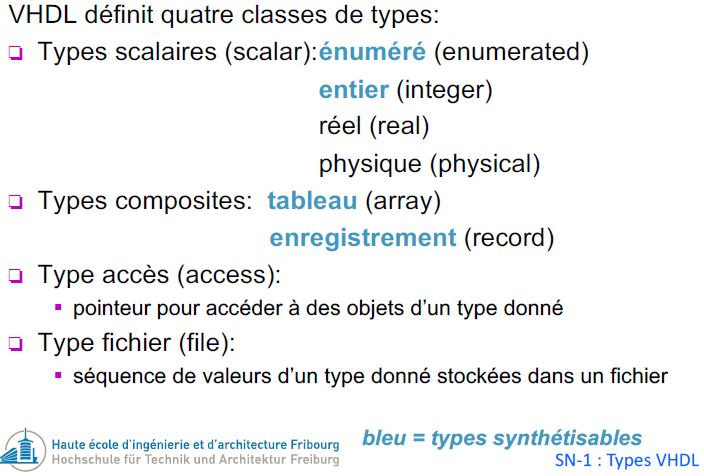
\includegraphics[scale=0.6]{1.JPG}\\[1.5cm]
            \vspace*{1\baselineskip}
            \today \\[0.7cm]
        \end{center}
    \end{titlepage}
    \tableofcontents
    \clearpage
% \insertImage{Img/1.PNG}{echelle pour l'image (source = 1)}{texte dessous l'image}{référence vers l'objet}
\section{Heure de travail}
12 heures

\section{Introduction}
Le but de TP est de pouvoir comprendre le fonctionnement d'une ligne série UART, d'un bus série I$^2$C et d'un bus série SPI. Ensuite de développer une ligne de commande sur l'interface série UART, de mettre en oeuvre le thermomètre sur le bus I$^2$C ainsi qu'un écran LCD sur le bus SPI afin de pouvoir implémenter tout ça comprendre comment étudier une datasheet d'un composant électronique simple
\section{Synthèse}

\paragraph{Sven}
\begin{itemize}
   \item Comment dessiner sur l'écran LCD
   \item Quand utiliser les pointeurs de fonctions
\end{itemize}

\paragraph{Marc}
\begin{itemize}
    \item Ce travail a été compliqué. le shell n'était pas trivial. Il y avait beaucoup de différentes méthodes, une architecture complexe et tout mettre ensemble n'est pas facile.
    \item Acquis mais à exercer: Les méthodes pour parser des inputs au clavier.  Il faudra aussi que je m'exerce sur les pointeurs qui était dans le cas du shell, pas facile à comprendre et à implémenter.
    \item Ce TP m'a toutefois permis de mieux comprendre le fonctionnement du beaglebone, malgré les problèmes rencontrés.
    \item compréhension de l'utilisation des différents périphériques tels que l'affichage LCD
\end{itemize}
 
\section{Quelles sont les caractéristiques principales (signaux et protocole) des interfaces de communication UART, I2C et SPI ?}
\paragraph{UART \(Universal Asynchronous Receiver/Transmitter\):} son but est de transmettre et recevoir les données depuis la ligne sérial. Son avantage est d'utiliser uniquement 2 fils pour transmettre les données\\
\begin{figure}[h!]
   \centering
   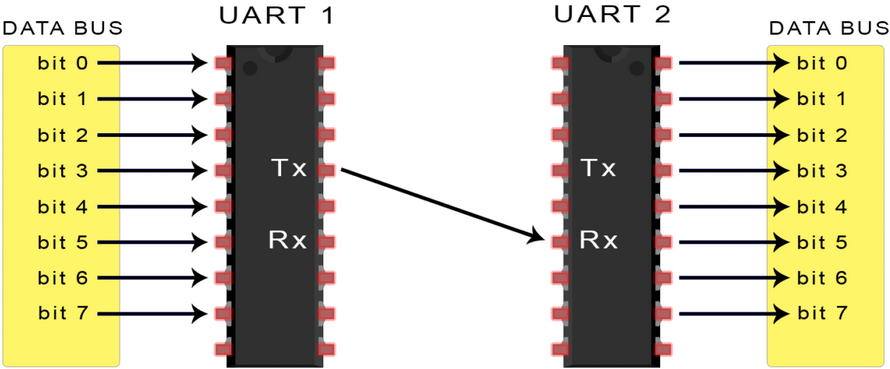
\includegraphics[width=.5\textwidth]{images/uart.png}
   \caption{UART}
\end{figure}

Les données sont transférées de manière asynchrone, il n'y a donc pas d'horloge, au moment de démarrer une transmission, la fréquence d'envoi est sélectionnée et exprimée en \textit{baud rate [bits par second]} c'est l'UART qui transmet va envoyer un seul bit pour démarrer la transmission et il va ensuite envoyer les 5 ou 9 bits de message avec un possiblité d'un bit de parité et va ensuite mettre la ligne de transmission sur haut pendant au moins de bit pour indiquer la fin de la transaction\\

Avantages
\begin{itemize}
   \item Utilise 2 fils
   \item Pas d'horloge
   \item bit de parité pour les erreurs
   \item Méthode efficace et prouvée
\end{itemize}

Désavantages
\begin{itemize}
   \item Taille maximum des données est de 9 bits
   \item Différence de baud rates entre les 2 UART doit être de 10\% 
\end{itemize}
 
\paragraph{SPI \(Serial Peripheral Interface\):} c'est un protocole de communication utilisé par exemple avec les lecteurs RFID et ils utilisent le SPI pour communiquer avec les microcontrollers. La transmission des données se fait avec un flux sans interruption donc les bits sont envoyés et reçus dans un flux continuz\\
\begin{figure}[h!]
   \centering
   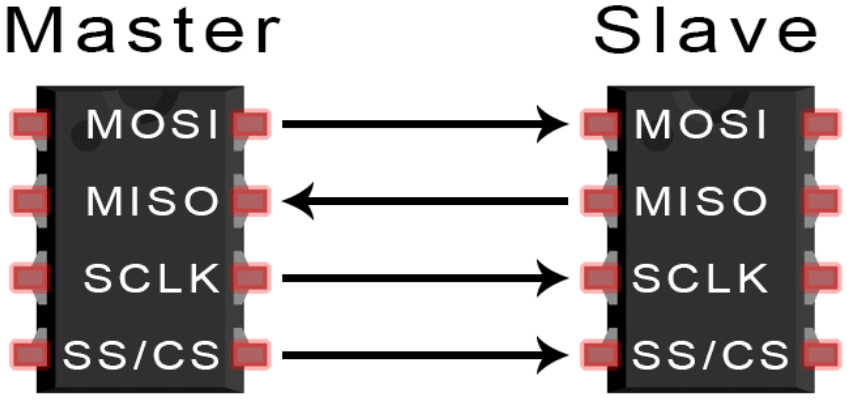
\includegraphics[width=.5\textwidth]{images/spi.png}
   \caption{SPI}
\end{figure}

Afin de pouvoir transmettre des données, il y a un master (microcontrolleur) et un slave (sensors) et il va recevoir les instructions du master, par exemple:
\begin{itemize}
   \item MOSI: ligne sur laquelle le maître envoie les données à l'esclave
   \item MISO: ligne sur laquelle l'esclave envoie les données au maitre
   \item SCLK: ligne pour l'horloge
   \item SS/ CS: utilisé si plusieurs slave, et permet de choisir vers qui envoyer les données
\end{itemize}
L'horloge (SCLK) permet de synchroniser l'envoi des bits au slave et c'est toujours le master qui démarre une transmission parce que c'est lui qui configure le signal d'horloge.\\
Ensuite il est possible de sélectionner plusieurs slave il faut donc décider avec qui il va discuter grâce à la pin SS, dans le cas d'un seul c'est slave la ligne va faire passe la ligne de bas à haut et va y rester. Dans le cas où plusieurs slave sont disponibles, il y 2 façons de les connecter: soit le master possède n SS pin qui seront connectées à chaque slave ou en utilisant un daisy-chained (les éléments sont chaînés les un aux autres) 
\begin{figure}[h!]
   \centering
   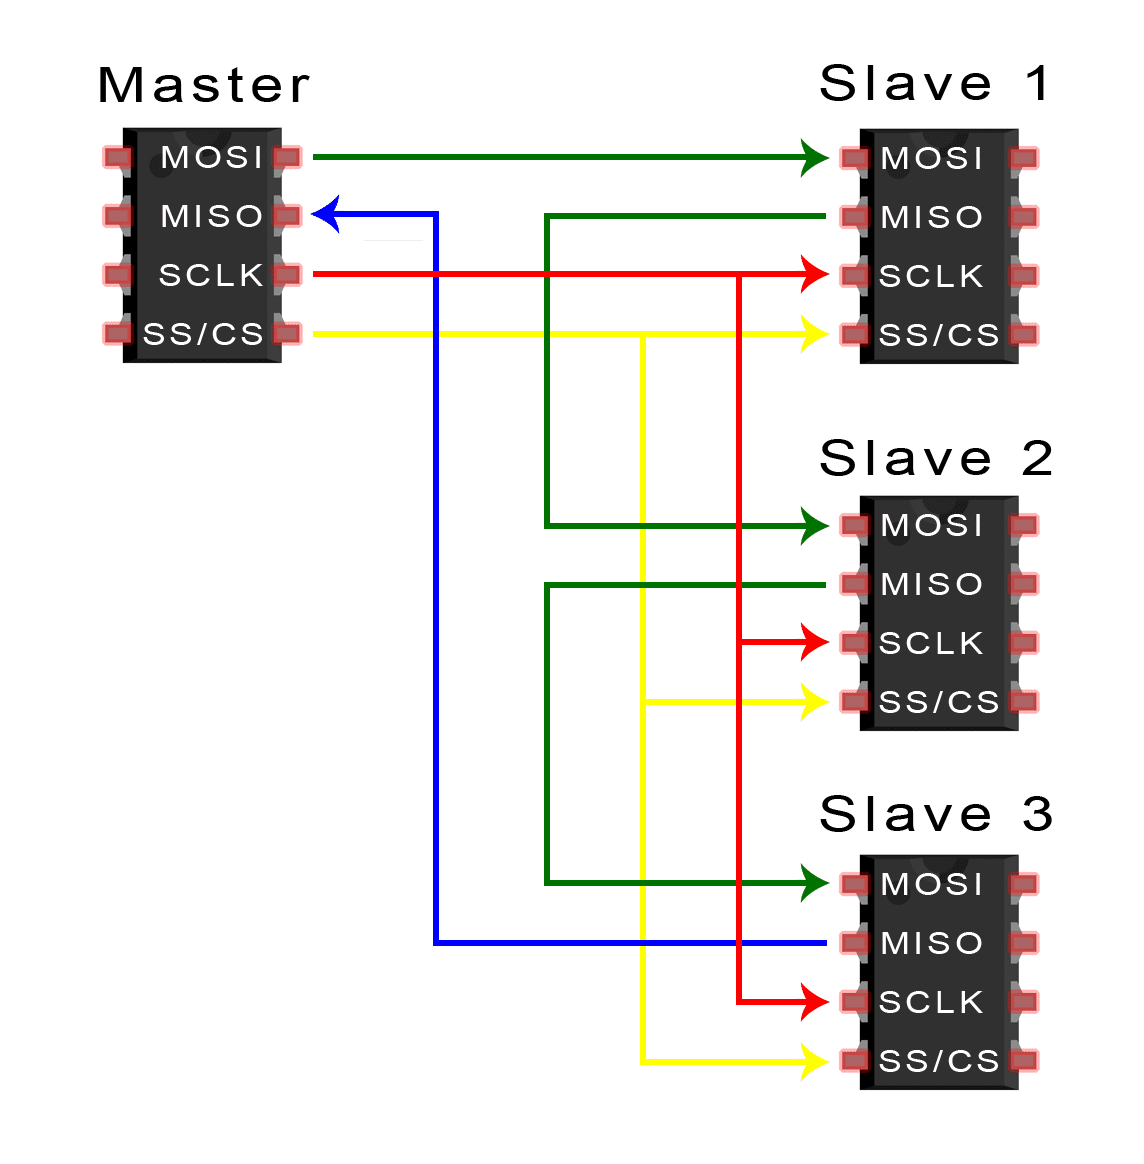
\includegraphics[width=.4\textwidth]{images/daisychained.png}
   \caption{Exemple de daisy-chained}
\end{figure}
Pour envoyer les informations, c'est la pin MOSI qui est utilisé à travers une ligne sérial et les bits sont envoyés les uns après les autres en commençant par le MSB et le slave peut lui aussi envoyer des informations, en commançant par le LSB en utilisant la pin MISO

Avantages
\begin{itemize}
   \item Flux continu sans interruption
   \item Adressage des slaves simple
   \item Taux de transfet rapide, dépend de la clk
   \item Informations peuvent être reçues et envoyées en même temps 
\end{itemize}

Désavantages
\begin{itemize}
   \item Utilise 4 fils
   \item Pas de contrôle si la donnée est correctement reçue
   \item Pas de bit de parité
   \item Uniquement un master
\end{itemize}

\paragraph{I2C \(Inter-Integrated Circuit \)}
Utilisé dans les OLED display (comme dans ce TP), gyroscope, etc et la différence entre le SPI c'est qu'il peut y avoir plusieurs master et il utilise uniquement 2 fils contrairement aux 4 d'avant
\begin{figure}[h!]
   \centering
   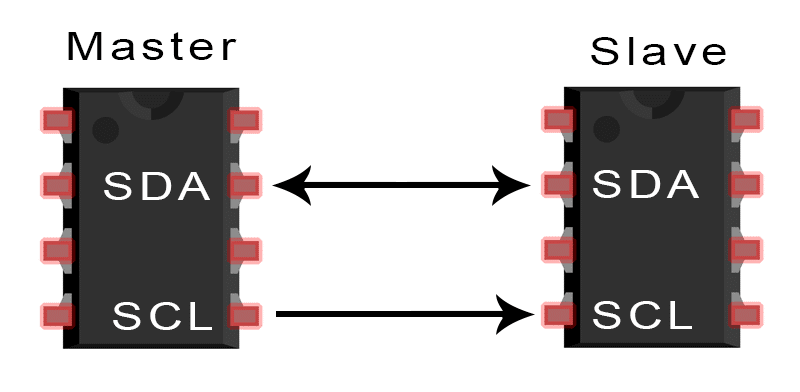
\includegraphics[width=.4\textwidth]{images/i2c.png}
   \caption{I$^2$C}
\end{figure}
Les pins qui sont utilisées sont:
\begin{itemize}
   \item SDA \textit{Serial Data}: ligne pour envoyer et recevoir les données entre le slave et le master
   \item SCL \textit{Serial Clock}: ligne qui transporte le signal de clock
\end{itemize}
Comme dans le SPI, la communication est synchrone grâce à l'horloge qui est contrôlée par le master.\\
Les données sont envoyées par frame, chaque message contient:
\begin{itemize}
   \item Start Condition: la ligne SDA passe de haut à bas avant que la SCL passe de haut à bas
   \item Stop Condition: la ligne SDA passe de bas à haut après que la SCL passe de bas à haut
   \item Address Frame: Identifie avec 7 à 10 bits, le slave auquel le master veut parler
   \item Read/ Write bit: permet au master en d'indiquer au slave qui lui envoie des données en mettant à 0 ou il attend d'en recevoir en passant à 1 
   \item ACK/ NACK bit: après chaque message, il est possible de savoir si la frame a bien été reçue
   \item data frame: contient le message codé sur 8 bits 
\end{itemize}
Dans le cas où il y a un master pour n slave il y a un minimum de 128 adresses et un maximum de 1024 adresses donc slave\\
Par contre avec ce protocole il possible d'avoir n master pour n slave, il se peut que 2 masters reçoive ou envoie des données sur la ligne SDA qui est partagée entre tous les composants (master+slave) du système donc pour palier à cela il faut que le master qui veut émettre des données doit d'abord détecter si la ligne SDA est haute ou basse avant de transmettre. Si la ligne est à l'état bas, un autre master à le contrôle et donc si la ligne est à l'état haut, le message peut être transmis

Avantages
\begin{itemize}
   \item Uniquement 2 fils
   \item Plusieurs master pour plusieurs slave
   \item Bit de confirmation si bien frame bien reçue
   \item Hardware moins compliqué que UART
   \item Protocole très utilisé
\end{itemize}

Désavantages
\begin{itemize}
   \item Taux de transfert plus bas que le SPI, Ultra fast mode = 5Mbps
   \item Taille d'une frame limitée à 8 bits
   \item Plus compliqué à intégrer que SPI
\end{itemize}

\section{Comment effectuer une rotation d'image avant d'être affichée sur un écran LCD ?}
Il est possible d'utiliser une matrice de rotation avec de retourner l'image avant qu'elle soit affichée
Dans notre cas, il faut faire une rotation de $90^{\circ}=\frac{\pi}{2}$\\
La formule de base est:
$$x'=x\cos(\frac{\pi}{2})-y\sin(\frac{\pi}{2})$$
$$y'=x\sin(\frac{\pi}{2})+y\cos(\frac{\pi}{2})$$
Et en sachant que $cos(-\frac{\pi}{2})=0$ et $sin(-\frac{\pi}{2})=1$, la solution pour effectuer une rotation est
$$x=-y$$
$$y=x$$ 


\section{Conclusion}
Nous n'avons pas pu terminer ce travail et cela vient du fait que nous n'avons pas bien compris comment utliser l'afficheur LCD fournis, nous allons donc dès que les solutions seront mises à disposition, travailler sur notre code afin de trouver ce qui nous empêchait d'avancer\\
Nous avons récupérer du code chez certains autres groupes afin de pouvoir mieux comprendre et avancer quelque peu.


\end{document}
